\documentclass[11pt,a4paper,twoside,headinclude,footexclude]{scrreprt}

%----------------------------------------------------------------------


% Language setting
% Replace `english' with e.g. `spanish' to change the document language
% \usepackage[english]{babel}

% Set page size and margins
% Replace `letterpaper' with `a4paper' for UK/EU standard size
%\usepackage[letterpaper,top=2cm,bottom=2cm,left=3cm,right=3cm,marginparwidth=1.75cm]{geometry}

% Useful packages
\usepackage{amsmath}
\usepackage{tikz}
\usetikzlibrary{trees}
\usetikzlibrary{positioning} 
\usetikzlibrary{arrows}
\usetikzlibrary{decorations.pathmorphing}
\usetikzlibrary{shapes.multipart}
\usetikzlibrary{shapes.geometric}
\usetikzlibrary{calc}
\usetikzlibrary{positioning} 
\usetikzlibrary{fit}
\usetikzlibrary{backgrounds}
\usetikzlibrary{automata}
\usepgflibrary{shapes.geometric}
\usetikzlibrary{shapes.geometric}
\usepackage{mathpartir}
\usepackage{listings}
\usepackage{proof}
\newtheorem{theorem}{Theorem}
\newtheorem{lemma}{Lemma}

\usepackage{graphicx}
%\usepackage[colorlinks=true, allcolors=blue]{hyperref}


\lstdefinelanguage{L4}
{morekeywords={
      assert 
    , class  
    , decl   
    , defn   
    , extends
    , lexicon
    , fact   
    , rule   
    , derivable
    , let   
    , in    
    , not   
    , forall
    , exists
    , if   
    , then 
    , else 
    , for  
    , true 
    , false
},    
sensitive=false,
morecomment=[l]{\#},
morestring=[b]",
}

\lstset{frame=tb,
  language=L4,
  aboveskip=3mm,
  belowskip=3mm,
  showstringspaces=false,
  columns=flexible,
  basicstyle={\footnotesize\ttfamily},
  numbers=none,
  numberstyle=\tiny\color{gray},
  keywordstyle=\color{blue},
  commentstyle=\color{green},
  stringstyle=\color{mauve},
  breaklines=true,
  breakatwhitespace=true,
  tabsize=2
}

%%% Local Variables: 
%%% mode: latex
%%% TeX-master: "main"
%%% End: 

% Theorems and definitions

% \newtheorem{definition}{Definition}
% \newtheorem{theorem}{Theorem}
% \newtheorem{lemma}{Lemma}
% \newtheorem{proposition}{Proposition}


% Definition of colors
\newcommand{\blue}[1]{{\color{blue}#1}}
\newcommand{\green}[1]{{\color{green}#1}}
\newcommand{\red}[1]{{\color{red}#1}}
\newcommand{\gray}[1]{{\color{gray}#1}}

% From MSCS file
\newcommand{\eg}{\textit{e.g.\ }}
\newcommand{\etal}{\textit{et al.\ }}
\newcommand{\etc}{\textit{etc}}
\newcommand{\ie}{\textit{i.e. }}
\newcommand{\viz}{\textit{viz.\ }}
\newcommand{\wrt}{\textit{w.r.t.\ }}
\newcommand{\lex}{\langle}
\newcommand{\rex}{\rangle}

% Own abbreviations
\newcommand{\secref}[1]{Section~\ref{#1}}
\newcommand{\secrefs}[1]{Sections~\ref{#1}}
\newcommand{\figref}[1]{Figure~\ref{#1}}
\newcommand{\figrefs}[1]{Figures~\ref{#1}}
\newcommand{\pgref}[1]{page~\pageref{#1}}
\newcommand{\theoremref}[1]{Theorem~\ref{#1}}
\newcommand{\theoremrefs}[1]{Theorems~\ref{#1}}
\newcommand{\lemmaref}[1]{Lemma~\ref{#1}}
\newcommand{\exampleref}[1]{Example~\ref{#1}}
\newcommand{\defref}[1]{Definition~\ref{#1}}

\newcommand{\figline}{\rule{\textwidth}{0.5pt}}


% Logique

\newcommand{\IMPL}[0]{\longrightarrow}
\newcommand{\IMPLL}[0]{\Longrightarrow} % another implication, to make
                                % a difference with reduction relations
\newcommand{\AND}[0]{\land}
\newcommand{\OR}[0]{\lor}
\newcommand{\NOT}[0]{\lnot}
\newcommand{\FALSE}[0]{\perp}
\newcommand{\TRUE}[0]{\top}
\newcommand{\IFF}[0]{\leftrightarrow}
\newcommand{\BIGAND}[1]{\bigwedge_{#1}}
\newcommand{\BIGOR}[1]{\bigvee_{#1}}
\newcommand{\BIGANDC}[2]{\bigwedge_{#1|#2}} % bigand with constraint
\newcommand{\BIGORC}[2]{\bigvee_{#1|#2}}    % bigor with constraint

\newcommand{\exgeq}[1]{\exists^{{\geq #1}}}
\newcommand{\exeq}[1]{\exists^{{= #1}}}
\newcommand{\exle}[1]{\exists^{{< #1}}}

% Remark macros for the authors

\newcommand{\remms}[2][]{\todo[color=green!40,#1]{MS: #2}}
\newcommand{\remre}[2][]{\todo[color=blue!40,#1]{RE: #2}}
\newcommand{\remjhb}[2][]{\todo[color=blue!20,#1]{JHB: #2}}


% Other

\newcommand{\smalltalcq}[0]{{\small small}-t{$\cal ALCQ$}}
\newcommand{\smalltalcqe}[0]{{\small small}-t{$\cal ALCQ$e}}
\newcommand{\trule}[0]{\xhookrightarrow}
\newcommand{\tableaurule}[1]{{\xhookrightarrow[]{#1}}}
\newcommand{\nodes}[1]{{\cal N}({#1})}
\newcommand{\trans}[1]{{\cal T}({#1})}
\newcommand{\transm}[1]{{\cal T'}({#1})}
\newcommand{\rconts}[1]{\llparenthesis #1 \rrparenthesis} %record contents
\newcommand{\rupd}[2]{{#1}\llparenthesis #2 \rrparenthesis} %record update

\newcommand{\eform}[0]{\mathit{eform}}
\newcommand{\form}[0]{\mathit{form}}
\newcommand{\free}[0]{\mathit{free}}
\newcommand{\exclprop}[0]{\stackrel{\times}{\longrightarrow}}

%%% Local Variables: 
%%% mode: latex
%%% TeX-master: "main"
%%% End: 


\RequirePackage{geometry}

\geometry{reset,twoside,a4paper,includemp=false,%
  top=4.5cm,bottom=4.5cm,left=3.2cm,right=3.2cm,%
  headheight=30pt
}

\begin{document}

%\textwidth 14cm

%\typearea[0.9cm]{10}
\pagestyle{fancyplain}
%\setcounter{tocdepth}{2}
%\renewcommand{\chaptermark}[1]{\markboth{\thechapter .\ #1}{\thechapter .\ #1}}
%\renewcommand{\sectionmark}[1]{\markright{\thesection\ #1}}
%\renewcommand{\chaptermark}[1]{\markboth{#1}{#1}}
%\renewcommand{\sectionmark}[1]{\markright{#1}}
%\lhead{\fancyplain{}{\em\leftmark}}
\lhead{}
%\rhead{\fancyplain{}{\em\rightmark}}
%\lfoot{}
%\lfoot{\small{\bf Initial Draft, \today}}
% \rfoot{\rm\thepage}
% \cfoot{}
%\setlength{\textfloatsep}{0cm}
%\setlength{\intextsep}{0cm}

%\addtolength{\topmargin}{1cm}







\begin{titlepage}

  \centering
\centerline{
\begin{minipage}[c]{5cm}
%\centerline{\includegraphics[scale=0.7]{LogoIRIT.jpg}}
\end{minipage}
\begin{minipage}[c]{5cm}
\centerline{
\includegraphics[scale=0.7]{logo-d-smu.jpg}}
\end{minipage}
\begin{minipage}[c]{5cm}
%\centerline{\includegraphics[scale=0.35]{logo_CNES.jpg}}
\end{minipage}
}
\ \vspace*{20mm}\\
  \begin{Huge}
    \textbf{L4 Language Report}\\
  \end{Huge}
\ \vspace*{4mm}\\
\ \vspace*{4mm}\\
\begin{LARGE}
  \centerline{{\today}}
  \ \vspace*{10mm}\\
  L4 Development Team
\end{LARGE}
\ \vspace*{5mm}\\
\begin{tabbing}
XXXXXX\=XXXXXXXXXXX \= \kill
\>                  \> \url{https://cclaw.smu.edu.sg/}
\end{tabbing}
\end{titlepage}

%----------------------------------------------------------------------
% Local Variables: 
% mode: latex
% TeX-master: "main"
% End: 


\cleardoublepage

%----------------------------------------------------------------------

%----------------------------------------------------------------------
\newpage
\tableofcontents
%\newpage
%\listoftables
\listoffigures

%----------------------------------------------------------------------
\cleardoublepage

%======================================================================

\chapter{User Documentation}

\section{Introduction}\label{sec:introduction}
\section{Introduction}\label{sec:introduction}

The goal of this paper is to show how a bottom up ASP reasoner like Clingo can be used for Abductive reasoning over First Order Horn clauses. As mentioned in the abstract previous work in abductive reasoning has mostly focused on implementing abduction in a top-down manner with Prolog as the underlying engine. CIFF \cite{mancarella09:_ciff} is a prominent example of this. More recently sCASP \cite{arias19:_const_answer_set_progr_groun_applic,arias_phd_2019} has been developed as a goal directed ASP implementation that can be used for abduction but this too uses a top down method for query evaluation. However there may be use cases where one wants to know all the resulting consequences of an abductive solution to a query with respect to a rule-set. Also, as mentioned in the abstract, top-down methods can sometimes result in solvers that are not truly declarative. Therefore an abductive reasoner that uses a solver like Clingo \cite{gebser12:_answer_set_solvin_pract} can
complement the abilities of goal directed reasoners like sCASP, CIFF \etc.

This paper shows how, given an input ASP rule set, one can write a new ASP program based on that rule set which will yield abductive solutions to queries, with the input ASP rule set as the background theory. The user does not have to explicitly specify the space of abducibles. This translation from the input ASP rule set to the derived ASP program is a purely mechanical one. The key idea is to encode backward chaining over the input rules through the use of meta predicates which incorporate a notion of 'reversing' the input rules to recursively generate pre-conditions from post conditions thereby generating a maximal space of abducibles. Then having generated this maximal space of abducibles, this 'feeds into' another part of the program where we have a representation of the input rules in the normal 'forward' direction. Entailment of the specified query is then checked via an integrity constraint and a minimal set of abduced facts is returned.

The main technical challenges are dealing with situations where input rules have existential variables in pre-conditions or when the query itself has existential variables. The other challenge is to control the depth of the abducibles generation process. The work that seems to come closest to ours is \cite{schueller16:_model_variat_first_order_horn}. It too uses some similar meta predicates to encode backward chaining, and a forward representation of the rules to check for query entailment via integrity constraints.

However there are several novel features in our work.  Firstly, depth  control for abducible generation is done in a purely declarative way as part of the encoding itself without needing to call external functions or other pieces of software. Furthermore, adding facts to the program automatically gives an implicit form of term substitution where Skolem terms or
other 'place-holder' terms occurring in abducibles are replaced away so that
the resulting proof is simplified, without any need for an explicit representation of equality between terms. Past work on this topic such as \cite{schueller16:_model_variat_first_order_horn} models equality between terms via an explicit equality predicate which may become unwieldy. Another approach to dealing with existential variables encountered during the abductive proof search is to simply ground all the rules over the entire domain of constants. However, this can often lead to too many choices for what an existential variable may be substituted for which may result in unexpected/unintuitive solutions. Our method avoids both of these techniques. We present three main sets of abductive proof generation encodings. One of the encodings only supports partial term substitution whereas the other two support full term substitution. Lastly, we also present an encoding which generates a set of directed edges representing a justification 
graph  for the generated proof, where the graph can be of any desired depth.

The rest of the paper is organised as
follows. First we give a brief introduction to Answer Set Programming and Abductive reasoning then, Section~\ref{sec:abductive_proof} defines the problem being tackled more formally. Section~\ref{sec:derived_asp} presents the encodings that facilitate the abductive proof generation and directed edge generation. The sections that follow discuss some formal results regarding completeness, finiteness of abductive proof generation. We also discuss a formal result regarding term substitution. Finally Section~\ref{sec:conclusion} discusses
future work and concludes.

This is an extended version of a paper presented at PPDP~2022 \cite{ppdp_version}.

\subsection{Answer Set Programming}
Answer Set Programming (ASP) is a declarative language from the logic programming family. It is widely used and studied by knowledge representation and reasoning and symbolic AI researchers for its ability to model common sense reasoning, model combinatorial search problems etc. It incorporates the $\textit{negation-as-failure}$ operator as interpreted under the $\textit{stable model semantics}$. Clingo is a well established implementation of ASP, incorporating additional features such as $\textit{choice rules}$ and optimization statements. We shall only briefly touch upon various aspects of ASP and Clingo here. The reader may consult \cite{gebser12:_answer_set_solvin_pract} for a more thorough description. Each rule in an ASP program consists of a set of body atoms. Some of these body atoms maybe negated via the negation as failure operator $not$. Rules with no pre-conditions are called facts. Given a set of rules $R$ and a set of facts $F$, the Clingo solver computes all stable models of the ASP program $F\cup R$. For example given the fact $r(alpha)$ and the rules:
\begin{lstlisting}[frame=none]
p(X):-r(X),not q(X).
q(X):-r(X), not p(X).
\end{lstlisting}
The solver will show us 2 models or answer sets given by\\ $\{r(alpha),p(alpha)\}$ and $\{r(alpha),q(alpha)\}$. Note that as opposed to Prolog, Clingo is a bottom up solver meaning that it computes complete stable models (also known as answer sets) given any ASP program. An integrity constraint is formally speaking a rule whose post-condition is the boolean $false$. In ASP, integrity constraints are written as rules with no post-conditions and are used to eliminate some computed answer sets. For example given in the following ASP program
\begin{lstlisting}[frame=none]
r(alpha).
p(X):-r(X),not q(X).
q(X):-r(X), not p(X).
:-q(X).
\end{lstlisting}
any answer set where some instantiation of $q$ is true is eliminated. Hence we get just one answer set. $\{r(alpha),p(alpha)\}$.\\ We will now give a quick introduction to two features of Clingo that we will use throughout this paper. Namely $\textit{choice rules}$ and $\textit{weak constraints}$. Weak constraints are also often known as optimization statements. Intuitively a choice rule is a rule where if the pre-conditions are satisfied then the post-condition may or may not be made true. The post-condition of a choice rule is enclosed in curly brackets. So given the following ASP program:\begin{lstlisting}[frame=none]
r(alpha).
{q(X)}:-r(X).
\end{lstlisting}, where the rule is a choice rule the solver will give us 2 models namely $\{r(alpha)\}$, $\{r(alpha),q(alpha)\}$. If we modify the program by adding an integrity constraint like so:
\begin{lstlisting}[frame=none]
r(alpha).
{q(X)}:-r(X).
:-q(X).
\end{lstlisting}
then we get just one model $\{r(alpha)\}$.\\
Weak constraints are used in Clingo to order answer sets by preference according to the atoms that appear in them. Without going into too much detail let us just explain the meaning of one kind of weak constraint which is the only kind that we will use in the paper namely:
\begin{lstlisting}[frame=none]
:~a(X). [1@1,X]
\end{lstlisting}
Adding this to an ASP program, orders the answer sets of the program according to the number of distinct instantiations of the predicate $a$ in the answer set. The answer set with the least number of instantiations of $a$ is called the most $optimal$ answer set. 
\subsection{Abductive Reasoning}
Briefly, abduction is a reasoning process where given a background theory $T$, we wish to find a set of facts $F$ such that $F\cup T$ is consistent and $F\cup T$ entails some goal $g$ for some given entailment relation. Usually we also want $F$ to be minimal in some well defined sense. Traditional Abductive Logic Programming has a long history, but we have our own definitions of what it means to formulate and solve an abductive reasoning problem and we will make all the relevant concepts/notions precise in the sections that follow.  


%%% Local Variables:
%%% mode: latex
%%% TeX-master: "main"
%%% End:



\section{L4 Language Overview}\label{sec:language}

%......................................................................
\subsection{Syntax}\label{sec:syntax}


%......................................................................
\begin{syntaxdiagram}{Program}
  \node[junction,right=of Program] (start) {};
  \node[junction,right=of start] (btle) {};
  \node[nonterminal,right=of btle] (TopLevelElement) {TopLevelElement};
  \node[junction,right=of TopLevelElement] (atle) {};
  \node[junction,right=of atle] (end) {$\diamond$};
  \node[junction,above=of TopLevelElement] (abfact) {};

\graph [use existing nodes] {
start -- btle -- TopLevelElement -- atle -> end
};

\syndiagBridge{atle}{abfact}{btle}
\end{syntaxdiagram}
%......................................................................


%......................................................................
\begin{syntaxdiagram}{TopLevelElement}
  \node[junction,right=of TopLevelElement] (start) {};
  \node[junction,right=of start] (btle) {};
  \node[nonterminal,right=of btle] (Mapping) {Mapping};
  \node[junction,right=of Mapping] (atle) {};
  \node[junction,right=of atle] (end) {};
  \node[nonterminal,below=of Mapping] (ClassDecl) {ClassDecl};
  \node[nonterminal,below=of ClassDecl] (GlobalVarDecl) {GlobalVarDecl};
  \node[nonterminal,below=of GlobalVarDecl] (GlobalVarDefn) {GlobalVarDefn};
  \node[nonterminal,below=of GlobalVarDefn] (Rule) {Rule};
  \node[nonterminal,below=of Rule] (Fact) {Fact};
  \node[nonterminal,below=of Fact] (Assertion) {Assertion};
  \node[nonterminal,below=of Assertion] (System) {System};

\graph [use existing nodes] {
start -- btle -- Mapping -- atle -> end
};

\syndiagAlternative{btle}{ClassDecl}{ClassDecl}{atle}
\syndiagAlternative{btle}{GlobalVarDecl}{GlobalVarDecl}{atle}
\syndiagAlternative{btle}{GlobalVarDefn}{GlobalVarDefn}{atle}
\syndiagAlternative{btle}{Rule}{Rule}{atle}
\syndiagAlternative{btle}{Fact}{Fact}{atle}
\syndiagAlternative{btle}{Assertion}{Assertion}{atle}
\syndiagAlternative{btle}{System}{System}{atle}

\end{syntaxdiagram}
%......................................................................

% %......................................................................
% \begin{syntaxdiagram}{Program}
%   \node[junction,right=of Program] (startl1) {};
%   \node[junction,right=of startl1] (bl) {};
%   \node[junction,right=of bl] (l) {};
%   \node[junction,right=of l] (al) {};
%   \node[junction,right=of al] (bcd) {};
%   \node[junction,right=of bcd,xshift=3mm] (cd) {};
%   \node[junction,right=of cd,xshift=3mm] (acd) {};
%   \node[junction,right=of acd] (bvd) {};
%   \node[junction,right=of bvd,xshift=7mm] (vd) {};
%   \node[junction,right=of vd,xshift=7mm] (avd) {};
%   \node[junction,right=of avd] (endl1) {$\cdots$};

%   \node[junction,below=of startl1,yshift=-10mm] (startl2) {};
%   \node[junction,right=of startl2] (brl) {};
%   \node[junction,right=of brl] (rl) {};
%   \node[junction,right=of brl] (rl) {};
%   \node[junction,right=of rl] (arl) {};
%   \node[junction,right=of arl] (bass) {};
%   \node[junction,right=of bass,xshift=3mm] (ass) {};
%   \node[junction,right=of ass,xshift=3mm] (aass) {};
%   \node[junction,right=of aass] (endl2) {$\diamond$};

%   \node[nonterminal,below=of l] (Lexicon) {Lexicon};
%   \node[nonterminal,below=of cd] (ClassDecls) {ClassDecls};
%   \node[nonterminal,below=of vd] (GlobalVarDecls) {GlobalVarDecls};
%   \node[nonterminal,below=of rl] (Rules) {Rules};
%   \node[nonterminal,below=of ass] (Assertions) {Assertions};
  
% \graph [use existing nodes] {
% startl1 -- bl -- l -- al -- bcd  -- cd -- acd -- bvd -- vd -- avd -> endl1
% };
% \graph [use existing nodes] {
% startl2 -- brl -- rl -- arl -- bass  -- ass -- aass -> endl2
% };

% \syndiagAlternative{bl}{Lexicon}{Lexicon}{al}
% \syndiagAlternative{bcd}{ClassDecls}{ClassDecls}{acd}
% \syndiagAlternative{bvd}{GlobalVarDecls}{GlobalVarDecls}{avd}
% \syndiagAlternative{brl}{Rules}{Rules}{arl}
% \syndiagAlternative{bass}{Assertions}{Assertions}{aass}
% \end{syntaxdiagram}


% \begin{syntaxdiagram}{Lexicon}
%   \node[junction,right=of Lexicon] (startl1) {};
%   \node[terminal,right=of startl1] (lexicon) {\texttt{lexicon}};
%   \node[junction,right=of lexicon] (bvar) {};
%   \node[terminal,right=of bvar] (var) {\emph{VAR}};
%   \node[terminal,right=of var] (arrow) {\texttt{->}};
%   \node[terminal,right=of arrow] (string) {\emph{string}};
%   \node[junction,right=of string] (astring) {};
%   \node[junction,right=of astring] (end) {};
%   \node[junction,above=of string] (abs) {};

% \graph [use existing nodes] {
% startl1 -- lexicon -- bvar -- var -- arrow -- string -- astring -> end
% };

% \syndiagBridge{astring}{abs}{bvar}
% \end{syntaxdiagram}
% %......................................................................


%......................................................................
\begin{syntaxdiagram}{ClassDecl}
  \node[junction,right=of ClassDecl] (start) {};
  \node[junction,right=of start,xshift=-3mm] (bdecl) {};
  \node[terminal,right=of bdecl,xshift=-3mm] (class) {\texttt{class}};
  \node[terminal,right=of class,xshift=-3mm] (classname) {\emph{VAR}};
  \node[junction,right=of classname,xshift=-4mm] (bextends) {};
  \node[terminal,right=of bextends,xshift=-4mm] (extends) {\texttt{extends}};
  \node[terminal,right=of extends,xshift=-3mm] (extendsname) {\emph{VAR}};
  \node[junction,right=of extendsname,xshift=-4mm] (bFields) {};
  \node[nonterminal,right=of bFields,xshift=-4mm] (Fields) {Fields};
  \node[junction,right=of Fields,xshift=-3mm] (aFields) {};
  \node[junction,right=of aFields,xshift=-3mm] (end) {};
%  \node[junction,above=of extends] (abextends) {};
  \node[junction,below=of extends] (blextends) {};

\graph [use existing nodes] {
start -- bdecl -- class -- classname -- bextends -- extends -- extendsname --
bFields -- Fields -- aFields -> end
};

%\syndiagBridge{aFields}{abextends}{bdecl}
\syndiagBridge{bextends}{blextends}{bFields}

\end{syntaxdiagram}
%......................................................................


%......................................................................
\begin{syntaxdiagram}{Fields}
  \node[junction,right=of Fields] (start) {};
  \node[junction,right=of start] (bleftbrace) {};
  \node[terminal,right=of bleftbrace] (leftbrace) {\verb|{|};
  \node[junction,right=of leftbrace] (aleftbrace) {};
  \node[nonterminal,right=of aleftbrace] (VarDecl) {VarDecl};
  \node[junction,right=of VarDecl] (brightbrace) {};
  \node[terminal,right=of brightbrace] (rightbrace) {\verb|}|};
  \node[junction,right=of rightbrace] (arightbrace) {};
  \node[junction,right=of arightbrace] (end) {};
  \node[junction,above=of VarDecl] (abVarDecl) {};
  \node[junction,below=of VarDecl] (blVarDecl) {};
  \node[junction,below=of blVarDecl] (blblVarDecl) {};

\graph [use existing nodes] {
start -- bleftbrace -- leftbrace -- aleftbrace -- VarDecl -- brightbrace --
rightbrace -- arightbrace -> end 
};

\syndiagBridge{brightbrace}{abVarDecl}{aleftbrace}
\syndiagBridge{aleftbrace}{blVarDecl}{brightbrace}
\syndiagBridge{bleftbrace}{blblVarDecl}{arightbrace}
\end{syntaxdiagram}
%......................................................................


%......................................................................
\begin{syntaxdiagram}{GlobalVarDecl}
  \node[junction,right=of GlobalVarDecl] (start) {};
  \node[junction,right=of start] (bdecl) {};
  \node[terminal,right=of bdecl] (decl) {\texttt{decl}};
  \node[nonterminal,right=of decl] (VarDecl) {VarDecl};
  \node[junction,right=of VarDecl] (aVarDecl) {};
  \node[junction,right=of aVarDecl] (end) {};

\graph [use existing nodes] {
start -- bdecl -- decl -- VarDecl -- aVarDecl -> end
};
\end{syntaxdiagram}
%......................................................................


%......................................................................
\begin{syntaxdiagram}{VarDecl}
  \node[junction,right=of VarDecl] (start) {};
  \node[junction,right=of start] (bvar) {};
  \node[terminal,right=of bvar] (var) {\emph{VAR}};
  \node[terminal,right=of var] (colon) {\texttt{:}};
  \node[nonterminal,right=of colon] (Tp) {Tp};
  \node[junction,right=of Tp] (aTp) {};
  \node[junction,right=of aTp] (end) {};

\graph [use existing nodes] {
start -- bvar -- var -- colon -- Tp -- aTp -> end
};
\end{syntaxdiagram}
%......................................................................



%......................................................................
\begin{syntaxdiagram}{GlobalVarDefn}
  \node[junction,right=of GlobalVarDefn] (start) {};
  \node[junction,right=of start] (bdefn) {};
  \node[terminal,right=of bdefn] (defn) {\texttt{defn}};
  \node[nonterminal,right=of defn] (VarDefn) {VarDefn};
  \node[junction,right=of VarDefn] (aVarDefn) {};
  \node[junction,right=of aVarDefn] (end) {};

\graph [use existing nodes] {
start -- bdefn -- defn -- VarDefn -- aVarDefn -> end
};
\end{syntaxdiagram}
%......................................................................


\remms{TODO}
%......................................................................
\begin{syntaxdiagram}{VarDefn}
  \node[junction,right=of VarDefn] (start) {};
  \node[junction,right=of start] (bvar) {};
  \node[terminal,right=of bvar] (var) {\emph{VAR}};
  \node[terminal,right=of var] (colon) {\texttt{:}};
  \node[nonterminal,right=of colon] (Tp) {Tp};
  \node[junction,right=of Tp] (aTp) {};
  \node[junction,right=of aTp] (end) {};

\graph [use existing nodes] {
start -- bvar -- var -- colon -- Tp -- aTp -> end
};
\end{syntaxdiagram}
%......................................................................



% %......................................................................
% \begin{syntaxdiagram}{Rules}
%   \node[junction,right=of Rules] (start) {};
%   \node[junction,right=of start] (brule) {};
%   \node[nonterminal,right=of brule] (Fact) {Fact};
%   \node[junction,right=of Fact] (arule) {};
%   \node[junction,right=of arule] (end) {};
%   \node[junction,above=of Fact] (abfact) {};
%   \node[nonterminal,below=of Fact] (Rule) {Rule};

% \graph [use existing nodes] {
% start -- brule -- Fact -- arule -> end
% };

% \syndiagBridge{arule}{abfact}{brule}
% \syndiagAlternative{brule}{Rule}{Rule}{arule}
% \end{syntaxdiagram}
% %......................................................................


%......................................................................
\begin{syntaxdiagram}{Rule}
  \node[junction,right=of Rule] (startl1) {};
  \node[terminal,right=of startl1] (rule) {\texttt{rule}};
  \node[terminal,right=of rule] (rname) {\texttt{<} \emph{VAR} \texttt{>}};
  \node[junction,right=of rname,xshift=-4mm] (bfor) {};
  \node[terminal,right=of bfor,xshift=-4mm] (for) {\texttt{for}};
  \node[junction,right=of for,xshift=-3mm] (bVarDecl) {};
  \node[nonterminal,right=of bVarDecl,xshift=-3mm] (VarDecl) {VarDecl};
  \node[junction,right=of VarDecl,xshift=-4mm] (aVarDecl) {};
  \node[junction,right=of aVarDecl,xshift=-4mm] (endl1) {$\cdots$};

  \node[junction,below=of startl1,yshift=-10mm] (startl2) {};
  \node[terminal,right=of startl2,xshift=-4mm] (if) {\texttt{if}};
  \node[nonterminal,right=of if,xshift=-3mm] (Expr1) {Expr};
  \node[terminal,right=of Expr1,xshift=-4mm] (then) {\texttt{then}};
  \node[nonterminal,right=of then,xshift=-3mm] (Expr2) {Expr};
  \node[junction,right=of Expr2,xshift=-3mm] (endl2) {};
  \node[junction,above=of VarDecl] (abVarDecl) {};
  \node[terminal,below=of VarDecl] (blVarDecl) {\texttt{,}};

\graph [use existing nodes] {
startl1 -- rule -- rname -- bfor -- for -- bVarDecl -- VarDecl -- aVarDecl -> endl1
};
\graph [use existing nodes] {
startl2 -- if -- Expr1 -- then -- Expr2 -> endl2
};

\syndiagBridge{bfor}{abVarDecl}{aVarDecl}
\syndiagBridge{aVarDecl}{blVarDecl}{bVarDecl}

\end{syntaxdiagram}
%......................................................................


%......................................................................
\begin{syntaxdiagram}{Fact}
  \node[junction,right=of Fact] (startl1) {};
  \node[terminal,right=of startl1] (fact) {\texttt{fact}};
  \node[terminal,right=of fact] (rname) {\texttt{<} \emph{VAR} \texttt{>}};
  \node[junction,right=of rname,xshift=-4mm] (bfor) {};
  \node[terminal,right=of bfor,xshift=-4mm] (for) {\texttt{for}};
  \node[junction,right=of for,xshift=-3mm] (bVarDecl) {};
  \node[nonterminal,right=of bVarDecl,xshift=-3mm] (VarDecl) {VarDecl};
  \node[junction,right=of VarDecl,xshift=-4mm] (aVarDecl) {};
  \node[nonterminal,right=of aVarDecl,xshift=-3mm] (Expr) {Expr};
  \node[junction,right=of Expr,xshift=-4mm] (endl1) {};
  \node[junction,above=of VarDecl] (abVarDecl) {};
  \node[terminal,below=of VarDecl] (blVarDecl) {\texttt{,}};

\graph [use existing nodes] {
startl1 -- fact -- rname -- bfor -- for -- bVarDecl -- VarDecl -- aVarDecl --
Expr -> endl1
};

\syndiagBridge{bfor}{abVarDecl}{aVarDecl}
\syndiagBridge{aVarDecl}{blVarDecl}{bVarDecl}
\end{syntaxdiagram}
%......................................................................


%......................................................................
\begin{syntaxdiagram}{Assertion}
  \node[junction,right=of Assertion] (start) {};
  \node[junction,right=of start] (bassert) {};
  \node[terminal,right=of bassert] (assert) {\texttt{assert}};
  \node[nonterminal,right=of assert] (expr) {Expr};
  \node[junction,right=of expr] (aexpr) {};
  \node[junction,right=of aexpr] (end) {};

\graph [use existing nodes] {
start -- bassert -- assert -- expr -- aexpr -> end
};

\end{syntaxdiagram}
%......................................................................


A \nonterminalref{Program} is the main processing unit. It consists of a
lexicon, a list of class declarations, global variable declarations, rules and
assertions, all of which can be missing.

A \nonterminalref{Lexicon} maps identifiers of the program to GF
strings\remms{Inari: more details}.

Class declarations (\nonterminalref{ClassDecl}) come in several shapes. In
its simplest form, a class declaration introduces a new class and relates it
to a superclass, as in
\begin{lstlisting}
class Lawyer extends Person
\end{lstlisting}  

The \texttt{extends} clause can also be omitted, in which case the superclass
is implicitly assumed to be \texttt{Class} (see \secref{sec:typing} for the
built-in class hierarchy). Thus,
\begin{lstlisting}
class Person
\end{lstlisting}  
is equivalent to:
\begin{lstlisting}
class Person extends Class
\end{lstlisting}

New fields can be added to a class with field declarations
(\nonterminalref{Fields}). These are variable declarations
enclosed in braces; they can also be missing altogether (equivalent to empty
field declarations \texttt{\{\}}). For example, 
\begin{lstlisting}
class Person {
   name : String
   age : Integer }

class Lawyer extends Person {
   companyName : String }
\end{lstlisting}  
introduces two fields \texttt{name} and \texttt{age} to class \texttt{Person},
whereas \texttt{Lawyer} inherits \texttt{name} and \texttt{age} from
\texttt{Person} and in addition defines a third field \texttt{companyName}.

Global variable declarations (\nonterminalref{GlobalVarDecl}) introduce names
that are meant to have global visibility in the program.

In the \nonterminalref{Rules} section, rules and facts can be mixed
arbitrarily. A \nonterminalref{Rule} introduces local variables in a
\texttt{for} clause (which may be omitted if there are no local variables),
followed by a precondition (\texttt{if}) and a postcondition (\texttt{then}),
both assumed to be Boolean expressions. If there are several preconditions,
these have to be conjoined by \emph{and} to form a single formula. 
A \nonterminalref{Fact} is a notational variant of a  \nonterminalref{Rule}
that does not have a precondition (more technically, a fact is mapped to a
rule whose precondition is \texttt{True}).

\nonterminalref{Assertion} are Boolean expressions introduced by the keyword \texttt{assert}.


%......................................................................
\subsection{Typing}\label{sec:typing}



%......................................................................
\subsection{Pragmatics}\label{sec:pragmatics}



%%% Local Variables:
%%% mode: latex
%%% TeX-master: "main"
%%% End:


\section{Specific Language Elements}\label{sec:language_elements}

%......................................................................
\subsection{Automata}\label{sec:automata}

Automata are an appropriate means for describing \emph{time-dependent} systems, as
opposed to rules and facts that provide a \emph{static} view.

In the present form, the L4 automata are inspired by the theory of Timed
Automata \cite{larsen1997uppaal} and in particular by the Uppaal
systen\footnote{\url{https://uppaal.org/}}. Our long-term aim is to go beyond the model
checking capabilities of Uppaal by a mapping of automata to SMT solvers. As
long as this feature is under development, we try to achieve maximal
compatibility so that Uppaal can be used together with L4, in two directions:

\begin{itemize}
\item The internal L4 data structures can be printed in the Uppaal
  \texttt{*.xta} format. An example is given in \figref{fig:system_uppaal}.
\item \texttt{*.xta} files written by Uppaal can be read by L4, with minor
  syntactic differences and restrictions. An example is given in \figref{fig:system_l4}.
\end{itemize}
The above automata are graphically displayed in \figref{fig:uppaal_automaton}.

\begin{figure}
\centering
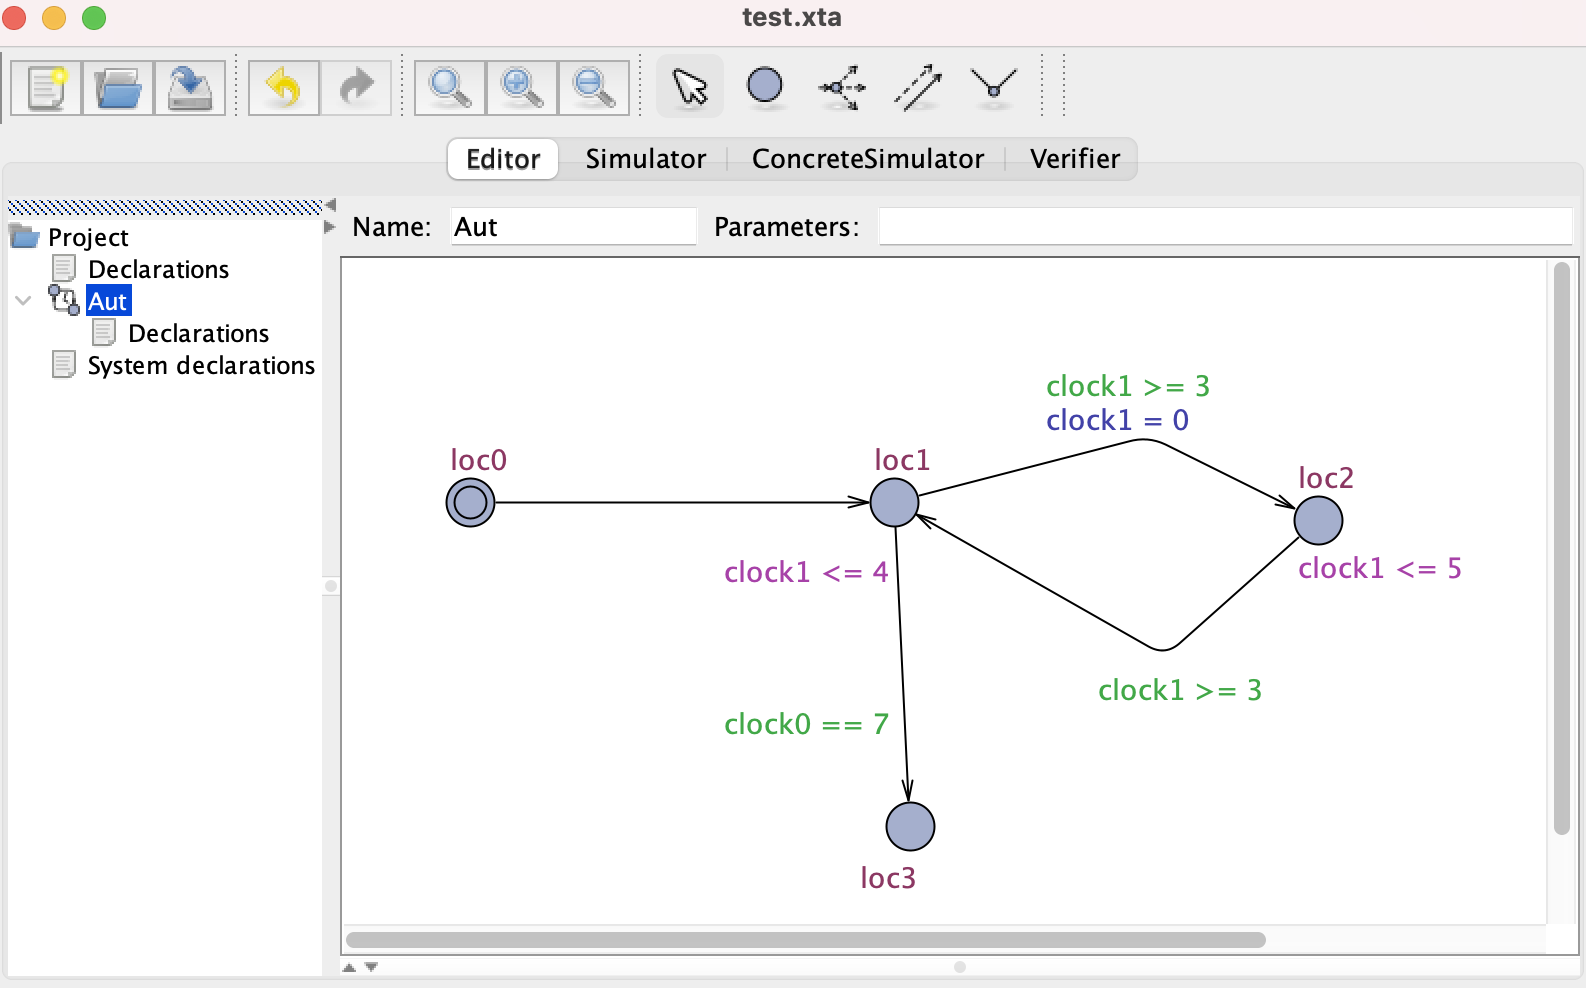
\includegraphics[scale=0.4]{Figures/uppaal_automaton.png}
\caption{Automaton represented in Uppaal}\label{fig:uppaal_automaton}
\end{figure}


These two methods will be revisited in the following.

\begin{figure}
  \begin{lstlisting}
chan x, y;
process Aut () {
    clock clock0, clock1;
    state
        loc0,
        loc1 { clock1 <= 4 },
        loc2 { clock1 <= 5 },
        loc3
        ;

    init loc0;
    trans
        loc1 -> loc3 { guard clock0 == 7 ;   },
        loc2 -> loc1 { guard clock1 >= 3 ;   },
        loc1 -> loc2 { guard clock1 >= 3 ;  assign clock1 = 0; },
        loc0 -> loc1 {    }
        ;
    }
system Aut; 
  \end{lstlisting}
  \caption{System specification in Uppaal format}\label{fig:system_uppaal}
\end{figure}

\begin{figure}
  \begin{lstlisting}
system AutSys {
    chan x, y;
    process Aut () {
        clock clock0, clock1;
        state
            loc0,
            loc1 { clock1 <= 4 },
            loc2 { clock1 <= 5 },
            loc3
            ;

        init loc0;
        trans
            loc1 -> loc3 { guard clock0 == 7 ;   },
            loc2 -> loc1 { guard clock1 >= 3 ;   },
            loc1 -> loc2 { guard clock1 >= 3 ;  assign clock1 = 0; },
            loc0 -> loc1 {    }
            ;
        }
    }
  \end{lstlisting}
  \caption{System specification in L4 format}\label{fig:system_l4}
\end{figure}



\subsubsection{Automata and Systems}

An \emph{automaton} is a graph commposed of nodes (states) and arcs
(transitions). States and transitions can be annotated with conditions
(temporal or not) and synchronization information. A \emph{system} is composed
of one or several automata and may contain declarations of channels (for
synchronization), clocks etc.


\subsubsection{From L4 to Uppaal}

The Uppaal \texttt{*.xta} format contains all the relevant structural
information for processing an automaton in Uppaal. However, no graphical
information is available, which typically leads to a poor layout when opening
an \texttt{*.xta} file.

An L4 program containing a system can be printed in Uppaal syntax with the
fake assertion
\begin{lstlisting}
  assert {printUp} True
\end{lstlisting}
which can be run as described in \secref{sec:running_solver}. The resulting
text can be written on a \texttt{*.xta} file and be processed by Uppaal. The
directive \texttt{printL4} produces the L4 format of automata.

Genuine proof obligations are currently not written to Uppaal (they would have
to be written to the corresponding \texttt{*.q} file).

\subsubsection{From Uppaal to L4}

A Uppaal \texttt{*.xta} file can be copied into L4 and then be manipulated as
any other L4 source. The L4 syntax and Uppaal syntax are sufficiently similar
so as to not require major changes, but the following manual postprocessing is
necessary:
\begin{itemize}
\item Automata and declarations belonging to one system have to be included
  into a system specification \texttt{system SysName \{ ... \}} as in
  \figref{fig:system_l4}. Several system specifications may coexist in an L4
  file.
\item Comments begin with a double slash (\texttt{//}) in Uppaal, which is not
  recognized by the L4 parser, and therefore have to be replaced by a sharp
  (\texttt{\#}) in L4.
\item Some expressions may be written differently, in particular the constants
  \texttt{True} and \texttt{False} which are written lowercase in Uppaal.
\end{itemize}

A notable difference is that Uppaal permits the declaration of automaton
\emph{templates} that can be instantiated. This is currently not possible in L4.



\remms[inline]{BEGIN TODO}
Note: there is another TODO file elsewhere. Integrate in this document, in a separate file to be excluded from compilation for the general public.
\begin{itemize}
\item local variable declarations not printed
\end{itemize}

\remms[inline]{END TODO}



%......................................................................
\subsection{Rules}\label{sec:rules}


%......................................................................
\subsection{SMT Solver}\label{sec:smt_solver}


\subsubsection{Assertions}\label{sec:assertions}


\subsubsection{Running the solver}\label{sec:running_solver}



%......................................................................
\subsection{Expert Systems}\label{sec:epert_systems}
\parskip=5pt plus 7pt
\parindent=15pt

Expert Systems are a way of replicating the logical reasoning and domain 
capabilities of a human expert through explicit knowledge capture.

L4 targets the use of expert systems as formal advisory interpreters; that form 
high-level conclusions given a set of ground truths and the application of formal 
axioms. 
\remal{There exists case-based legal expert systems, but my personal opinion is that these are less intuitive and much harder to support} 
Legal texts are typically well-structured \& formal, with well-defined 
terms integrated in clear and specific domains. However, there might be 
situations where the interpretive ability of a trained lawyer are required, 
but cannot be accessed due to the insufficient time or resources. Situations like
these are prime areas that expert systems excel in. Unfortunately,  
previous attempts at legal-specific expert systems in the 1980s and 1990s were 
largely exploratory and descriptive in nature, with no attempts at public testing. \cite{leith2016riseandfall}

In the time since, there have been various efforts into the building of rigorous 
and efficient rule-based systems.
\remal{To cite drool's rete, find clara's paper (if it exists) etc.} 
To build on the results of these efforts, we offer L4 as an upstream format that 
transpiles to such existing formats. 

As with existing expert systems, L4 files already mimic the characteristics 
of an easily modifiable knowledge base. 
Furthermore, this approach allows you, the user-developer/knowledge engineer, 
the option of choosing the language environment you would like to work with, and the 
flexibility of desigining a frontend user interface that would fit your purposes.

The currently supported rule-engine output formats are 
\href{https://docs.jboss.org/drools/release/7.58.0.Final/drools-docs/html_single/}{Drools} 
and 
\href{http://www.clara-rules.org/}{Clara-Rules}.



%%% Local Variables:
%%% mode: latex
%%% TeX-master: "main"
%%% End:


%======================================================================
\chapter{Developer Documentation}

\section{Parsing and Typechecking}\label{sec:parsing_typechecking}
Describes the parsing technlogy and typechecking procedures

%%% Local Variables:
%%% mode: latex
%%% TeX-master: "main"
%%% End:



\section{Translations to Proof and Reasoning Tools}\label{sec:translations}
Describing the translations to tools such as sCasp, Z3, \dots

%%% Local Variables:
%%% mode: latex
%%% TeX-master: "main"
%%% End:


%======================================================================
\chapter{Internal}
\todo[inline]{Attention, this chapter should be commented out for publication of the document}

%----------------------------------------------------------------------
\section{TODO}
%----------------------------------------------------------------------

The following issues are still unresolved

%----------------------------------------------------------------------
\section{Collection of thesis / internship topics}
%----------------------------------------------------------------------

Collection of ideas for subprojects with CCLAW


%%% Local Variables:
%%% mode: latex
%%% TeX-master: "main"
%%% End:


%======================================================================
\newpage
\bibliographystyle{alpha}
\bibliography{main}

\end{document}

%%% Local Variables:
%%% mode: latex
%%% TeX-master: t
%%% End:
